% Train-time ablation section, v2 (2026-09-23): adds the "w/o failure experience" arm (ABL-Q8-NOLAST, docs/01) to the
% user's current text. Figure = fig_ablation_v2.pdf (plot_ablation.py --v2), table = sec_ablation_appendix_v2.tex
% (tab_ablation.py --v2). The new arm is ONE attacker run so far; when run 2 (seed 2048) is in, add it to NOLAST_RUNS in
% plot_ablation.py, regenerate both, and update the three numbers marked <<r2>> below plus "a single attacker training".

\subsubsection{Train-Time Ablation of Self-Reflection}
\label{sec:train_time_ablation}

To isolate the contribution of self-reflection reasoning during training, we fine-tune Qwen3-8B on the same attacked agentic trajectories and expert actions without self-reflection reasoning supervision, following the same SR-Agent training recipe. We evaluate the resulting model under RL-Hammer adaptive attack. To account for a possible mismatch between training and inference, we report two settings for the ablated model: one with thinking enabled, following the standard evaluation protocol used for Qwen3-8B and SR-Agent, and one with thinking disabled. For each setting, the target configuration is kept fixed throughout both attacker training and evaluation.

This first ablation removes the reflection as a whole, so it cannot tell whether the gain comes from the failure experience specific to SRFT or from safety-oriented reasoning supervision in general. We therefore train a second ablated model, \emph{w/o failure experience}, whose reflection keeps the first two components of Template~2 --- the summary of the original goal and the identification of the injected instruction --- but omits the third, the safety-aware action analysis that contrasts the expert action with the agent's own sampled candidate actions and their consequences. Everything else is unchanged: the same trajectories, the same expert actions, the same recipe, and the same evaluation protocol as SR-Agent, with thinking enabled.

\begin{figure}[t]
  \centering
  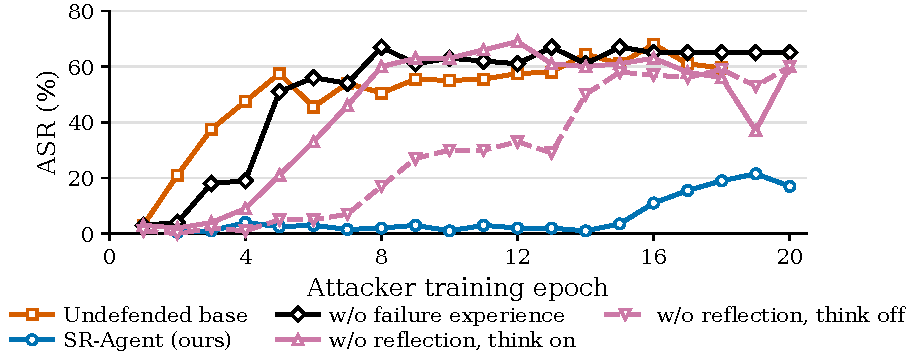
\includegraphics[width=0.72\linewidth]{fig_ablation_v2.pdf}
  \caption{\textbf{Train-time ablation of self-reflection under adaptive attack (Qwen3-8B).}
  The \emph{w/o failure experience} model is trained with the goal summary and injection identification kept and the action analysis over the agent's own candidate actions removed; the two \emph{w/o reflection} curves use the same checkpoint and differ only in whether thinking is enabled at inference.}
  \label{fig:train_time_ablation}
\end{figure}

As shown in Figure~\ref{fig:train_time_ablation}, removing self-reflection supervision largely eliminates the adaptive robustness gained by SRFT. The ablated model reaches a final ASR of $60.0\%$ with thinking enabled and disabled, closely matching the undefended Qwen3-8B at $59.5\%$. In contrast, SR-Agent achieves a substantially lower final ASR of $17.0\%$. Removing only the failure experience is just as damaging: the \emph{w/o failure experience} model reaches a final ASR of $65.0\%$ % <<r2>>
and is already above $50\%$ by the fifth attacker epoch, while SR-Agent stays below $5\%$ at the same point; its peak of $67.0\%$ % <<r2>>
is reached at epoch 8. % <<r2>>
Exact per-epoch values and endpoint statistics are provided in Table~\ref{tab:train_time_ablation}.

Notably, the two \emph{w/o reflection} settings exhibit nearly identical final vulnerability despite using different inference modes. This suggests that the degradation is not explained by whether the model is explicitly encouraged to reason at test time. Rather, the key difference lies in the training signal itself: exposure to attacked trajectories together with supervision on the correct action is insufficient to reproduce the robustness of SRFT.

The second ablation locates this signal. The two components that the \emph{w/o failure experience} model retains --- restating the task objective and naming the injected instruction --- are exactly what a generic safety-oriented chain of thought would provide, and on their own they leave the model as exposed as no reflection at all. What the adaptive attacker cannot overcome is the third component: the analysis of the actions the agent itself was drawn to under attack and of their consequences. The robustness of SRFT therefore rests on learning from the agent's own failure experience rather than on reasoning supervision in general, which is the distinction the method is built on.
